\section{Contexto}
Este Trabajo de Fin de Grado (en adelante, TFG) consiste en el diseño e implementación de una aplicación web para el estudio y comparación de actividades deportivas, principalmente actividades de carrera. La aplicación, denominada \textit{ATRA}, permite a los usuarios analizar su desempeño en distintas actividades, agrupar actividades en función de la ruta que recorren, y comparar varias actividades simultáneamente.  Adicionalmente, ofrece ciertos aspectos sociales, permitiendo la creación de murales, comunidades en las que varios usuarios pueden compartir actividades y comparar su desempeño con el de sus amigos.

La aplicación será utilizada por deportistas que buscan estudiar su desempeño a lo largo del tiempo, o que buscan una herramienta para comparar su desempeño en distintas ocasiones. Estos deportistas, al salir a correr, utilizan aplicaciones como Strava, SportsTracker,  o MapMyRun para grabar la actividad. Luego, pueden exportar los datos grabados e introducirlos en ATRA para su estudio y análisis.

La motivación para llevar a cabo este proyecto surge del interés personal del autor, así como del potencial académico que ofrece desarrollar una aplicación de este estilo. Si bien existen muchas aplicaciones que ofrecen funcionalidades de grabación y análisis de actividades, y muchas de ellas son mucho más completas de lo que busca conseguir esta aplicación, no se ha podido encontrar una solución que considere todas las funcionalidades objetivo y las haga disponibles de forma gratuita. Por tanto, se ha tomado la decisión de desarrollar una solución personalizada, de forma que pueda tener exactamente las funcionalidades buscadas. 

Además, desarrollar una aplicación web es un ejercicio académico valioso que se cimienta en habilidades desarrolladas durante la carrera, a la vez que requiere profundizar más en las tecnologías y procedimientos estudiados para poder ser completada satisfactoriamente. De esta manera, ofrece una oportunidad de expandir conocimientos y habilidades, a la vez que se gana familiaridad con tecnologías y herramientas utilizadas en el mundo laboral.


\section{Estado del arte}
Antes de desarrollar cualquier producto nuevo, es necesario estudiar la situación del mercado para identificar posibles huecos, así como familiarizarse con las funcionalidades ofrecidas por otras aplicaciones, tanto para que sirvan de base para saber qué funcionalidades implementar, como para identificar posibles huecos en las funcionalidades ofrecidas, que puedan ser ocupados por la aplicación desarrollada.

Esta sección resume este estudio de mercado, comentando varias de las aplicaciones estudiadas y las funcionalidades que ofrecen.

\subsection{Strava}
Strava es la aplicación más popular para grabación y estudio de actividades deportivas, dada su amplia comunidad de atletas, así como su ecosistema de aplicaciones y extensiones. Ofrece soporte para carreras, caminatas, ciclismo, senderismo, y muchas más actividades.

Permite crear actividades mediante grabación directa o importando archivos desde distintos formatos. En su versión gratuita ofrece análisis básico, incluyendo ritmo por kilómetro, gráficas de altura y ritmo medio, y una sección de \textit{Best Efforts} con los mejores tiempos en distancias fijas. También incluye funcionalidades sociales, como la comparación de resultados en rutas o segmentos y la notificación de récords personales o globales.

La versión de pago añade análisis más avanzados, como la distribución del ritmo, comparación del rendimiento en una ruta, y creación de rutas.
\begin{figure}[H]
    \centering
    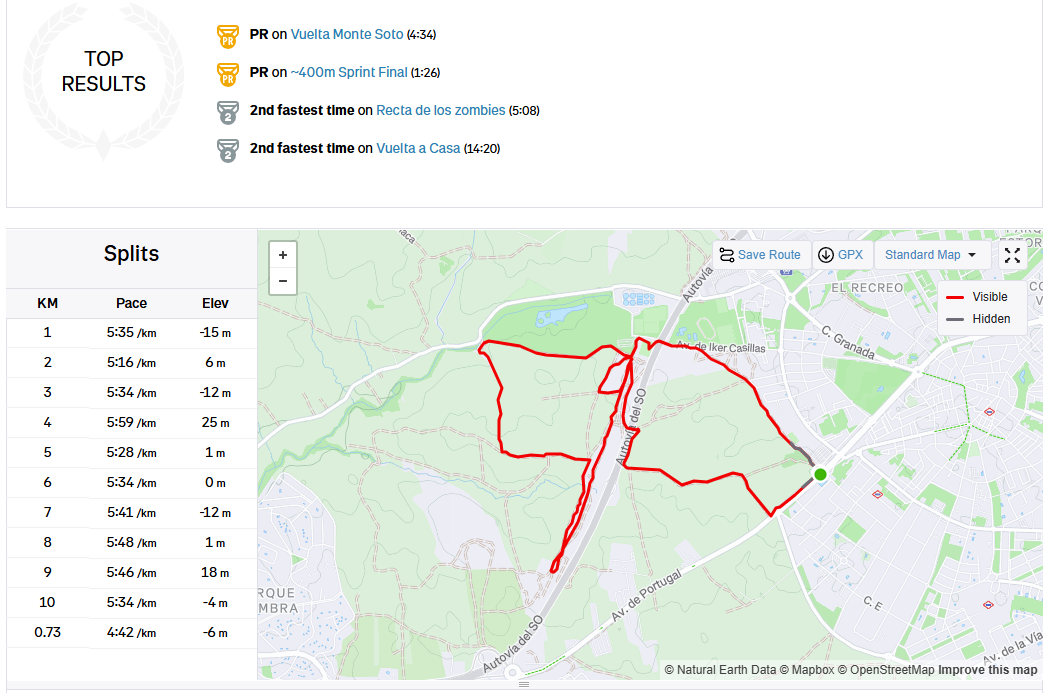
\includegraphics[width=0.5\linewidth]{img/Strava_dashboard.png}
    \caption{Análisis de Actividad en Strava}
    \label{fig:strava}
\end{figure}

Aunque Strava destaca por su comunidad y sus funcionalidades sociales, su versión gratuita ofrece capacidades limitadas de análisis y comparación de actividades. Además, su enfoque se centra principalmente en el seguimiento social y competitivo, más que en el análisis detallado de datos. Por ello, aunque es una referencia en este ámbito, no cubre completamente los objetivos planteados en este proyecto.

La plataforma de Strava está accesible en la url \href{https://www.strava.com/}{\uline{strava.com}\footnote{\url{https://www.strava.com/}}}, y se puede leer sobre la aplicación en su sección \href{https://www.strava.com/about}{\uline{About Us}\footnote{\url{https://www.strava.com/about}}}.

\subsection{VeloViewer}
VeloViewer es una aplicación web de estudio detallado de actividades construido a partir de la API de Strava. No permite la creación de actividades ni rutas, sino que se conecta con Strava y utiliza las actividades y datos almacenadas en Strava para generar visualizaciones, gráficos, y realizar distintos cálculos. Como indica el nombre, el enfoque está centrado en visualización, ofreciendo varias funcionalidades avanzadas de visualización. Permite ver la ruta de una actividad en 3d con un "auto-runner" que la recorre a un ritmo proporcional al ritmo original, gráficos de líneas sincronizados para cada métrica, junto con diagramas de bigotes y barras, histogramas mostrando la distribución de valores de cada métrica, gráficos de calor, de dispersión, de líneas, y otros, permitiendo además cambiar qué representa cada eje en los gráficos, herramientas de visualización de la dirección de movimiento durante la actividad, y otras tantas visualizaciones avanzadas. 

Las visualizaciones comentadas funcionan para una actividad determinada, pero VeloViewer también ofrece visualizaciones para grupos de actividades. Permite generar y descargar una infografía comparando las métricas como distancia total o elevación total con distancias entre ciudades o la altura de monumentos o montes, un calendario mostrando la actividad a lo largo del año, gráficos de líneas de la distancia acumulada, y un gráfico de barras mostrando la distancia cubierta por día/semana/mes/año. Además, la página principal ofrece tablas con información acumulativa de interés, como distancia/tiempo/elevación total, número de actividades, máxima distancia/elevación/tiempo en una única actividad, récords de distancia, actividades recientes,  y más.
\begin{figure}[H]
    \centering
    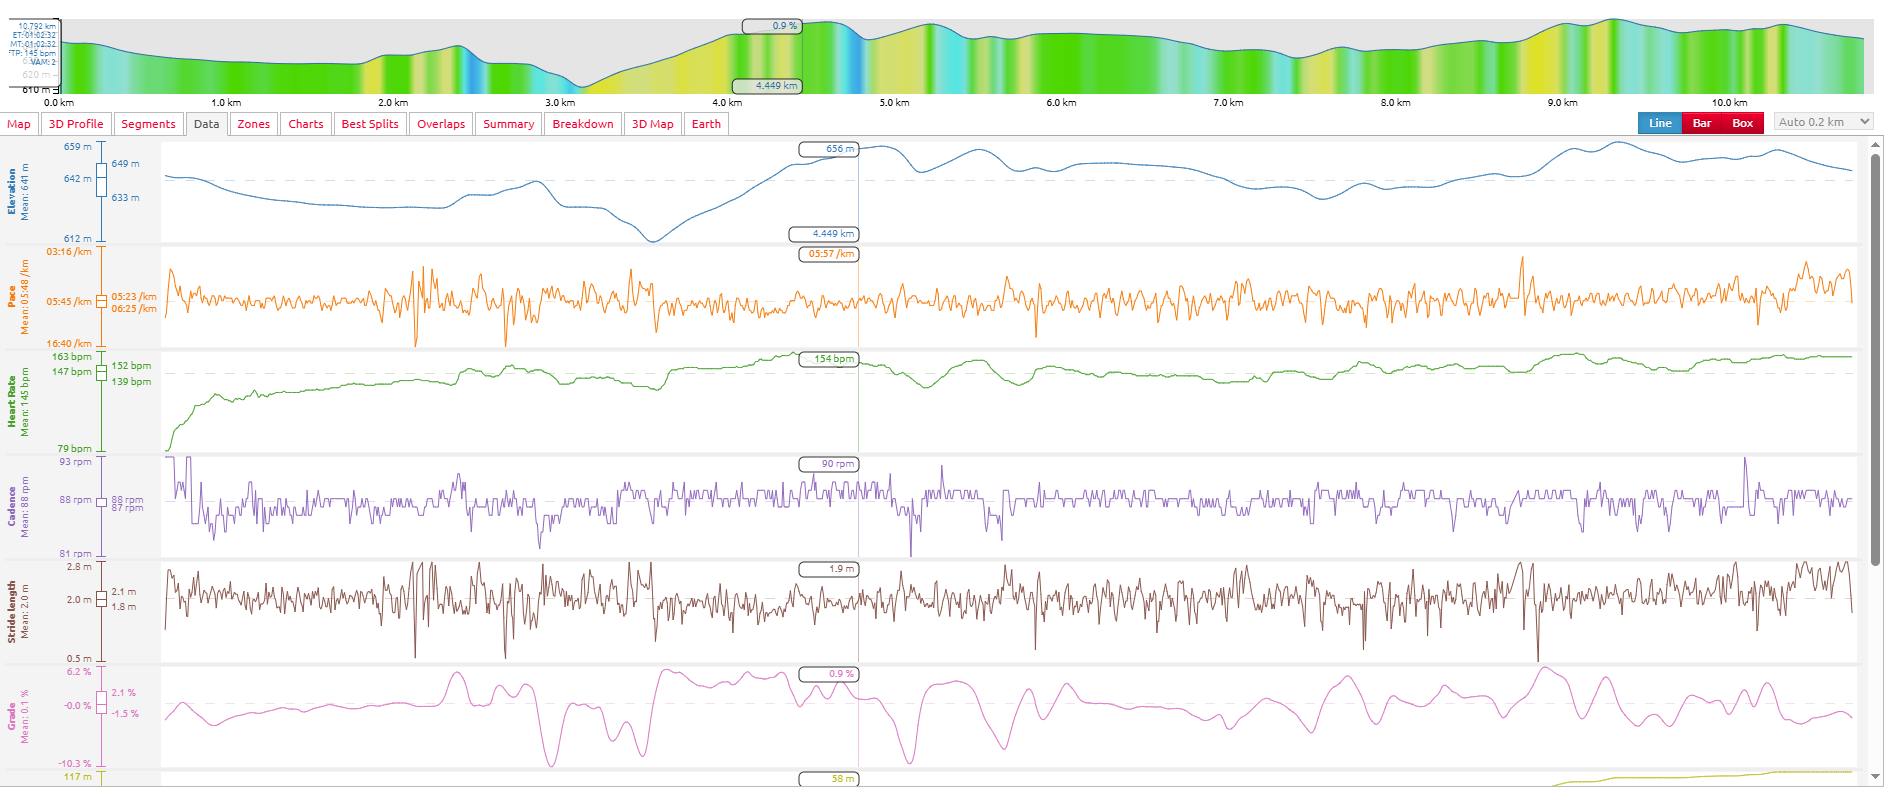
\includegraphics[width=0.5\linewidth]{img/VeloViewer.png}
    \caption{Análisis de Actividad en VeloViewer}
    \label{fig:VeloViewer}
\end{figure}

La figura \ref{fig:VeloViewer} muestra la pestaña \textit{Data} de la visualización de una actividad en la aplicación VeloViewer. En ella, se pueden ver las distintas gráficas que ofrece, así como el resto de pestañas disponibles. Notable destacar que permite cambiar el tipo de gráfico entre líneas, de barras, y cajas y bigotes. El resto de pestañas ofrecen las funcionalidades descritas anteriormente, así como otras no discutidas.

VeloViewer es una herramienta excelente para el estudio de actividades individuales, así como para la visualización del progreso a lo largo del tiempo, gracias a las funcionalidades como el calendario o las distintas gráficas que muestran el progreso acumulado durante el año. Ofrece una suite muy completa de visualizaciones sobre los datos generados en las actividades realizadas. Sin embargo, no permite la comparación directa de actividades, ni el estudio de datos acumulados en un subconjunto de actividades seleccionadas por el usuario. Por tanto, aunque es una herramienta muy potente, y muchas de sus funcionalidades se han tomado como referencia durante el diseño de la aplicación, el enfoque de estas funcionalidades en la visualización y estudio de actividades individuales implica que no ofrece capacidades de comparación de actividades, por lo que no cubre totalmente los requisitos del proyecto.

La aplicación VeloViewer es accesible en \href{https://veloviewer.com/}{\uline{veloviewer.com}\footnote{\url{https://veloviewer.com/}}}. Sin embargo, esa página da acceso a la herramienta, para lo que es necesario iniciar sesión con Strava. En su lugar, se puede consultar información sobre la herramienta en \href{https://blog.veloviewer.com/about/}{\uline{blog.veloviewer.com/about}\footnote{\url{https://blog.veloviewer.com/about/}}}.

\subsection{MapMyRun}
MapMyRun es una aplicación de grabación y análisis de actividades, popular por su simplicidad y funcionalidades de seguimiento de progreso y creación de objetivos y planes de entrenamiento. Permite la grabación y estudio de actividades, además de contar con aspectos comunitarios y una amplia variedad de retos en los que participar.

Permite la creación de actividades mediante grabación de las mismas, así como importando archivos en varios formatos, y manualmente, seleccionando una ruta e introduciendo el resto de datos. También permite la creación de rutas, ya sea manualmente, seleccionando puntos en el mapa, o a partir de una actividad realizada. Sin embargo, no ofrece un listado de actividades en una ruta determinada, ni funcionalidades que aprovechen la agrupación.

En cuanto al estudio de las actividades, ofrece funcionalidades básicas, calculando distancia total, ritmo medio, y otras métricas genéricas. Además,  permite visualizar un gráfico de líneas mostrando altura y ritmo frente a tiempo transcurrido o distancia, permitiendo al usuario cambiar entre esas dos métricas. Por último, ofrece un mapa interactivo que muestra la ruta tomada dividida en secciones de distancia configurable, junto con una lista detallando el ritmo medio durante cada sección.
\begin{figure}[H]
    \centering
    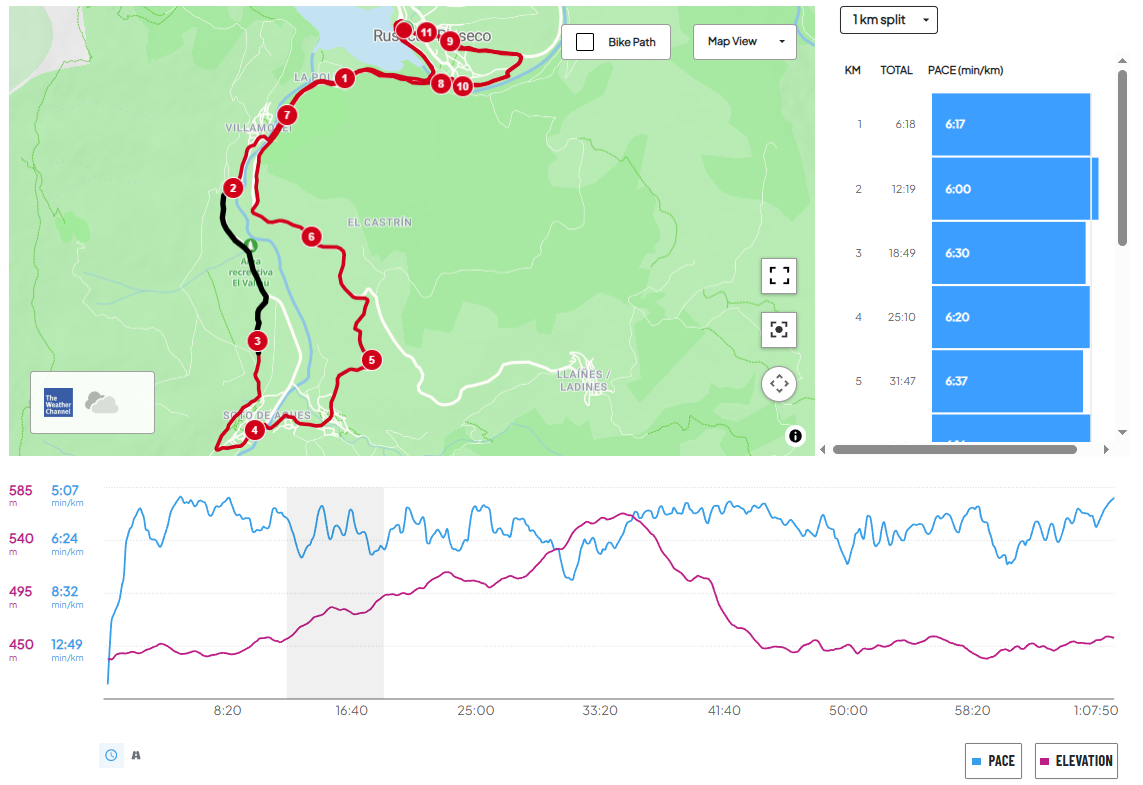
\includegraphics[width=0.5\linewidth]{img/MapMyRun.png}
    \caption{Análisis de Actividad en MapMyRun}
    \label{fig:MapMyRun}
\end{figure}

En la figura \ref{fig:MapMyRun} se pueden ver las herramientas de visualización que ofrece la aplicación. De especial interés es la posibilidad de modificar la longitud de las particiones mediante el botón desplegable encima de la lista, pudiendo elegir visualizar secciones de 0.1, 0.5, 1, 5, ó 10 kilómetros.

En lo referente a aspectos sociales, ofrece una sección comunidad, donde puedes ver actividades de otros usuarios o de amigos. 

También ofrece una suite de otras funcionalidades, que, si bien son de menor interés para el enfoque de este proyecto, constituyen el principal atractivo de la aplicación para sus usuarios. Entre estas funcionalidades encontramos la capacidad de conectarse con dispositivos como relojes o zapatillas inteligentes, la creación de planes de entrenamiento personalizados, y la disponibilidad y seguimiento de distintos retos en los que puedes participar para mantener la motivación.

En resumen, MapMyRun es una aplicación de grabación de actividades con un enfoque más centrado en ayudar a los atletas a mantener la motivación y seguir planes de entrenamiento que en el estudio detallado de actividades concretas y su comparación con otras. Por esto, se considera que no cubre los requisitos del proyecto.

\subsection{Conclusión}
Tras haber realizado un estudio de varias aplicaciones en este espacio, se ha llegado a la siguiente conclusión: si bien existen muchas aplicaciones distintas que permiten grabación de actividades, y su posterior estudio y análisis, ofreciendo visualizaciones complejas, no se ha encontrado una aplicación que ofrezca comparación de actividades, o funcionalidades como análisis de la distribución del ritmo, al menos no como parte de la versión gratuita de la aplicación. Por tanto, se considera que el desarrollo de la aplicación está justificado, ya que cubre un hueco existente en el mercado, al ofrecer funcionalidades de comparación de actividades y análisis de la distribución de manera gratuita.

\section{Objetivos}
Esta sección recoge los objetivos funcionales y técnicos del proyecto definidos en las primeras fases del mismo.

\subsection{Objetivos funcionales} 
Los objetivos funcionales describen las capacidades que debe tener la aplicación. Son funcionalidades de alto nivel que aportan valor a los usuarios y diferencian la aplicación de otras. Se centran en torno a la creación de actividades a partir de un archivo GPX, y al posterior análisis de las actividades creadas, así como la comparación de varias actividades distintas. Además, también es importante que la aplicación ofrezca un método para juntar actividades que hayan ocurrido en la misma ruta, así como para ver actividades de otros usuarios y compararlas con las propias. 

\noindent Se plantean los siguientes objetivos funcionales:

\begin{table}[H]
\centering
\small
\begin{tabularx}{\textwidth}{@{} X X @{}}
% La "X" hace que las columnas se repartan el ancho al 50% automáticamente
\textbullet{} Crear actividad desde archivo GPX. & \textbullet{} Agrupar actividades en una ruta. \\ \addlinespace
\textbullet{} Analizar actividad y su distribución. & \textbullet{} Comparar actividades en la misma ruta. \\ \addlinespace
\textbullet{} Visualizar gráficos con datos. & \textbullet{} Compartir actividades en murales. \\ \addlinespace
\textbullet{} Visualizar actividad en un mapa. & \\ 
\end{tabularx}
\end{table}

\subsection{Objetivos técnicos}
Los objetivos técnicos describen cómo debe ser desarrollada la aplicación. Especifican las tecnologías que se deben utilizar en cada parte de la aplicación y para cada funcionalidad. El objetivo técnico principal es desarrollar una aplicación web con \textit{frontend} SPA y \textit{backend} API REST. Para ello, se utilizarán los frameworks Angular y Spring Boot. Además, se realizará un empaquetado y despliegue automático de la aplicación, aplicando principios de CI/CD. Para ello, se hará uso de Docker, Azure, y GitHub Actions. Además, para garantizar la calidad del código, se realizarán pruebas de calidad mediante pruebas con JUnit y Selenium, y análisis estático con SonarQube. 

\noindent Se plantean los siguientes objetivos técnicos:


\begin{table}[H]
\centering
\small
\begin{tabularx}{\textwidth}{@{} p{0.45\textwidth} p{0.45\textwidth} @{}}
\textbullet{} Desarrollar frontend SPA con Angular & \textbullet{} Realizar CI/CD con GitHub Actions \\
\textbullet{} Desarrollar API REST con Spring Boot & \textbullet{} Desplegar la aplicación en Azure \\
\textbullet{} Empaquetar la aplicación con Docker & \textbullet{} Implementar pruebas con JUnit, Selenium y Mockito \\
& \textbullet{} Realizar análisis de código con SonarQube \\
\end{tabularx}
\end{table}
